\chapter*{Introduction}
\addcontentsline{toc}{chapter}{Introduction}
\markboth{Introduction}{Introduction}
\label{chap:introduction}
%\minitoc

Dans le cadre de notre cursus en Master Informatique à Lille 1, nous avons eu l’opportunité de réaliser un projet sur l’ensemble du semestre appelé PJI. Chaque étudiant ou binôme pouvait choisir un sujet sur lequel travailler parmi une liste mais également proposer le sien.
Nous avons choisi de nous intéresser à un sujet proche de l'informatique embarquée, qui est un domaine grandissant à l'aube de l'Internet des Objets. Notre sujet se porte sur la détection de paquets falsifiés dans un réseau 6LoWPAN.

\begin{figure}[htp]
	\centering
	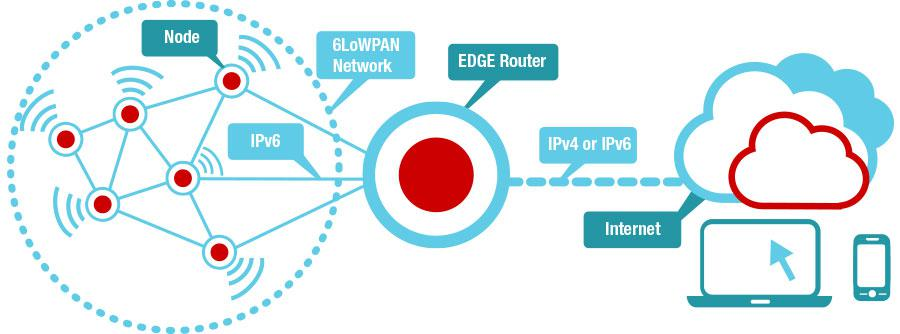
\includegraphics[width=16cm]{images/6lowpan.jpg}
	\caption{Diagramme d'explication de 6LoWPAN.}
	\label{fig:diagramme-6lowpan}
\end{figure}
L'équipe proposant ce sujet est le groupe 2XS \textbf{eXtra Small eXtra Safe} composée de notamment \textbf{Gilles GRIMAUD} notre encadrant, \textbf{Michael HAUSPIE} son collègue proche de ce sujet et bien sûr le reste de l'équipe.

%%% Local Variables: 
%%% mode: latex
%%% TeX-master: "isae-report-template"
%%% End: 
